\documentclass[a4paper]{article}

\usepackage[utf8]{inputenc}
\usepackage{graphicx}
\usepackage{subfig}

\begin{document}

\title{DH2323: Lab 1}
\author{Karl Johan Andreasson \and Erik Fahlén}

\maketitle
\clearpage

\section{Methods}
Because we both initially thought that this lab seemed to be quite simple, we started by doing two separate approaches and then comparing them.
These were then merged into a final solution.
After that we made some final bugfixes and added some new functionality, such as motion blur in the star field.

We tried to make the solutions as elegant as possible.
Both of us have taken the C++ course (DD2387), so we are quite comfortable from using C++ components such as templates, iterators and new features from the C++11 standard.

When we started merging our projects, we chose to start using some proper version tracking, with git.
This helped our work substantially, and was something that carried on to the other labs.

\section{Discussion}
The gradient interpolation we thought was very easy.
Rather than making two separate functions for floats and vectors, we extended the first implementation to use C++ templates.
We really liked this solution, since it limits the amount of code.
With this part of the lab, we had very few problems, it pretty much worked the first time we compiled it.

The star field was slightly more challanging.
Projecting 3D points to the screen was not that easy, mostly because we did not remember the math behind it very well.
Once we got that working, it was rather easy to adjust the velocity to get nice movement.
Making the particles wrap around was also not that difficult once we had the movement working.

We found the concept of motion blur in the star field to be the most complicated to do in this lab.
One initial approach was to have a number of positions for each star, representing different stages of placement between the current frame and the last frame.
This looked fine when animated, but when looking at the screenshots, it was obvious that the stars were not continous lines, especially near the camera.

Because of these problems, we moved on to drawing a line for each star.
The line is drawn between the star's previous position and the current position.
The only exception is when the stars wrap around.
There the previous position is manually reset to the current position.
If we were not to do this there would occationally be lines all the way from the star's starting point to its end point.

While this approach looked much better, is was more complicated to implement.
We had to research line-drawing algorithms, which turned out to be quite extensive field.
The algorithm that we ended up using were actually a composition of our own.
While it is probably not the most efficient algorithm, it is quite elegant from a mathematical point of view.
It works by calculating a normalized direction vector for the line and stepping with it to fill in the required pixels.
The line is also clipped where the screen ends to not drop performance.

We also discovered that these line actually did not look good at high frame rates.
Because the star moved such a short distance for each frame, the blur effect was barely visible.
We solved this by simply limiting the frames per second to 30.
This also has the benefit that the application is not as heavy for the CPU, since it can sleep for a while after drawing each frame.

\section{Results}
The result from the gradient interpolation can be seen in figure \ref{gradient_fig}.
You can clearly see the smooth transition between the interpolated colors.
In the middle of the frame, all four colors blend together into a greyish color.

\begin{figure}[H]
\begin{center}
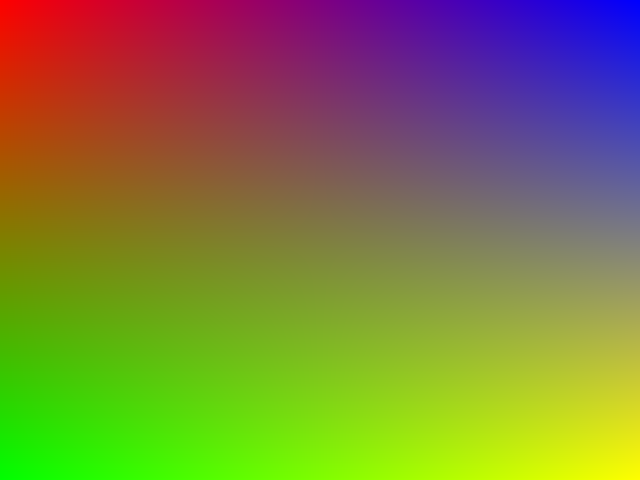
\includegraphics[width=\textwidth]{gradient.png}
\caption{Gradient produced by interpolation}
\label{gradient_fig}
\end{center}
\end{figure}

The star field is shown in figure \ref{starfield_fig}.
There are a few more things to say about the star field.
First of all, note that the screenshot shown here does not quite do the animation justice, obviously.
You can see some of the motion blur in the edges.
These are the stars that are closest to the camera, which is way they have the longest blur lines.
The bottom left corner is probably the place where this is most visible.
Also not that all motion blur lines are directed out from the image.
This really helps to sell the effect that we are moving through the star field.

\begin{figure}[H]
\begin{center}
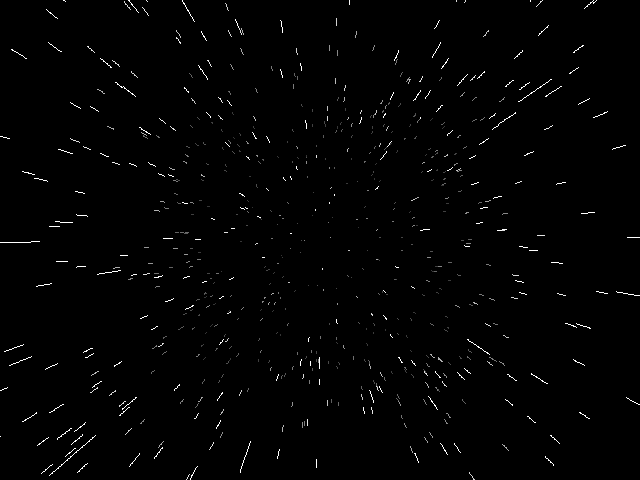
\includegraphics[width=\textwidth]{starfield.png}
\caption{star field with motion blur}
\label{starfield_fig}
\end{center}
\end{figure}
\end{document}
